% Evangelos 2009/12/19

\subsection{\label{s:mfReqb}\CLe\  general linear \slice}

The use of the simple, irreducible subspace \slice\ condition in \refsect{s:cleCoordSlice},
\refeq{cLeCoordSlice} allowed explicit and straightforward determination of invariant
variables \refeq{eq:invLaser}. Unfortunately the moving frame method introduced artificial
singularities in \reducedsp, the location of which depends on the choice of slice point,
as we've seen in \refsect{sec:CLeMovFr}.
Therefore we examine in this section how different, less restrictive choices of slice fixing
point affect the singular set. The price to pay is that it won't be convenient (although not
impossible for our simple example) to explicitly write out transformations
to invariant variables as we did in \refsect{sec:mf};
we will instead implement the moving frame map numerically,
mapping computed trajectories to the \slice.
This is not a serious limitation. Even though analytical computation
of invariants with the {\mframes} is efficient, it is still
prohibitive for very high dimensional flows. For, one has
to compute the invariants with computer algebra, a proccess
that works\rf{SiminosThesis} for moderate system dimension of the order of $100$,
as required for instance in truncations of \KSe\ studied in \refref{SCD07},
but does not scale well for problems with truncations of order $10,000$ as
a fully resolved $3$-D fluid simulation would easily require\rf{GibsonPhD}.
Furthermore, in order to analyze the singularities present in the system, \refeq{cLeMFsing}
describing the singular subspace is all we need to know.

Since \REQB{1} organizes reduced space dynamics around it, but also sets the
scale of angular velocity of symmetry induced rotations in the system, we
find natural to choose slice-fixing point $\slicep=(0,\,1,\,y_1^{o}/x_2^{o},\,x_1^{o}/x_2^{o},\,y_2^{o}/x_2^{o},\,0)$
with $\ssp^{o}= \ssp_{\REQB{1}}=$\ES{Fill this in.}, \ie\ on the group orbit of \reqv.
We can use \refeq{cLeMF} to compute $\theta$ for any point $\ssp$, but keeping up
with the numerical approach of this section, we use a Newton's method. As initial
guess we use the angle from previous point along the trajectory, while for the
first point we choose among the two possible solutions by demanding that the rotation
results to a point at minimum distance from \slicep.
Projections of \cLf\ to the slice defined in this manner are
shown in \reffig{fig:CLEmf}\,(b).
The figure exhibits clearly the moving frame angle $\pi$-jumps.

To visualize the \sset\ we eliminate $x_2$ in \refeq{cLeMFsing} to obtain
\beq
	\slicepComp{y}{1}x_2+\slicepComp{y}{2}x_1+\left(\slicepComp{y}{2}+\slicepComp{y}{1}^2\right)y_1\,=0.
\ee{cLeMFsingElim}
We plot the projection of \sset\ in $3$-dimensions
$(x_1,x_2,y_1)$ in \reffig{fig:CLEmfsset}(a). We observe the
attractor meet the \sset\ head on and become deformed.
    \ES{Axes are wrong in figure, I'll fix this.
	}

Linear relation \refeq{cLeMFsingElim} and
\reffig{fig:CLEmfsset} suggest that we can manipulate the
\sset\ so that the attractor avoids the singularity by
increasing the ratio $\slicepComp{y}{2}/\slicepComp{y}{1}$.
Choosing slice fixing point as
$\slicep=\ssp_{\REQB{1}}+(0,-5,0,0,0)$
    \ES{With updated notation this choice of \slicep\ does not
    make sense but I will have to replot the figures before I can
    update it.}
we can therefore ``tilt'' the \sset\ so that
trajectories approach it in a smoother manner, see
\reffig{fig:CLEmfsset}\,(b).
    \ES{I've updated figure \reffig{fig:CLEmfAdHoc}
	to compare $(x_1,y_1,z)$ projection with the two different choices.
	I'm not sure that the plot of the singular set is accurate in this
	projection though. To me the difference is clear here, the image
	system in the second case is as smooth as with invariant polynomials.
       }
     \PC{I combined the two figures, removed \reffig{fig:CLEmfAdHoc}.
     \\
     no need to say "a slice orthogonal to the group tangent". For our
     linear slices it is so by construction.
     }
%%%%%%%%%%%%%%%%%%%%%%%%%%%%%%%%%%%%%%%%%%%%%%%%%%%%%%%%%%%%%%%%
%computed with vaggelis/testing/flows/CLEfinalTmp.nb
\begin{figure}[ht]
\begin{center}
  (\textit{a})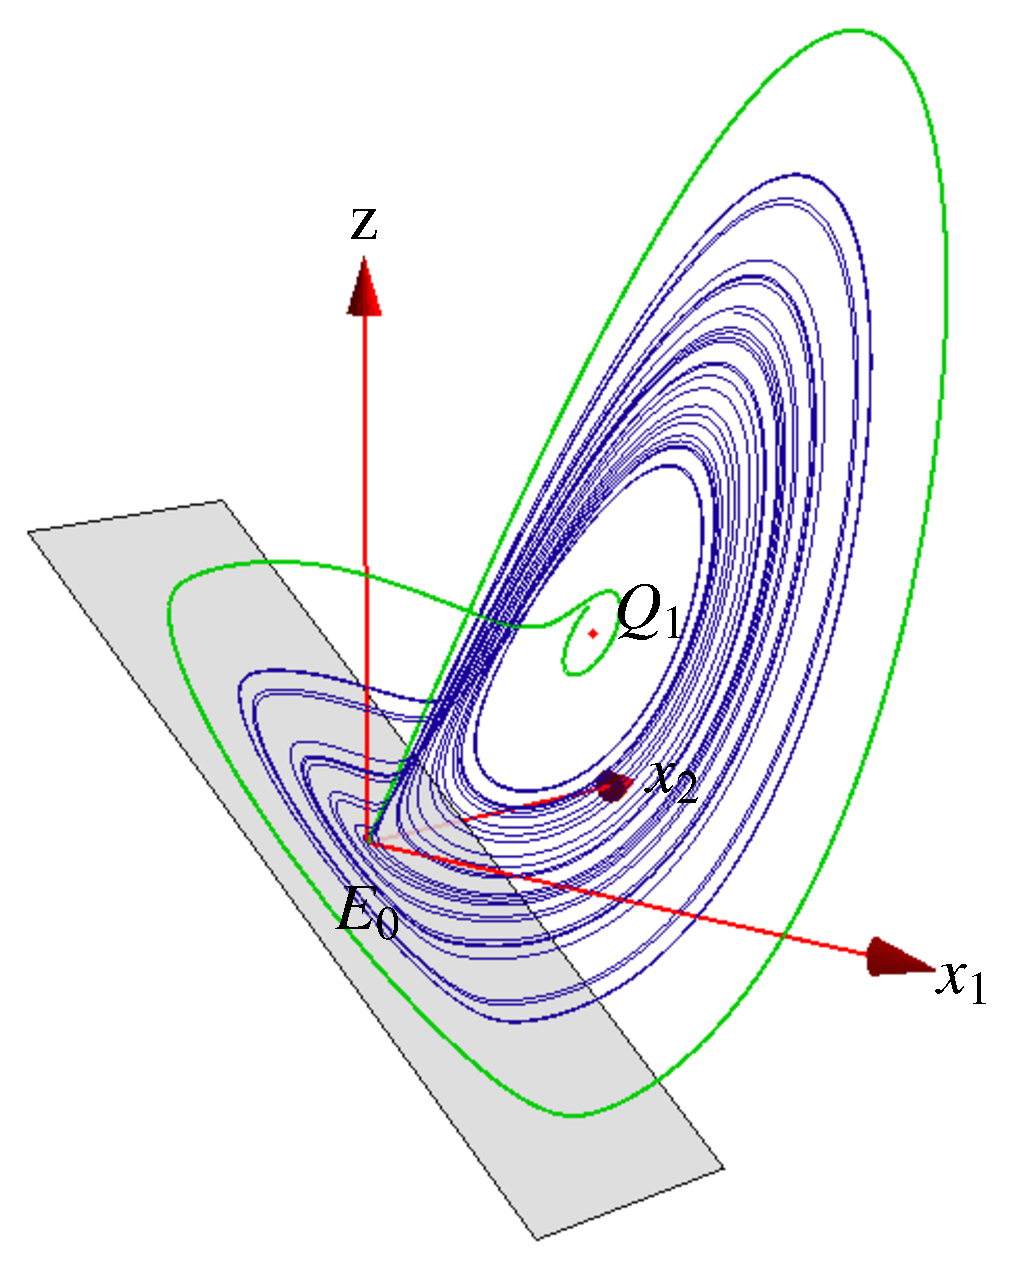
\includegraphics[width=0.35\textwidth,clip=true]{CLEmfReqb123}
~~~~(\textit{b})%
% PC eliminated: 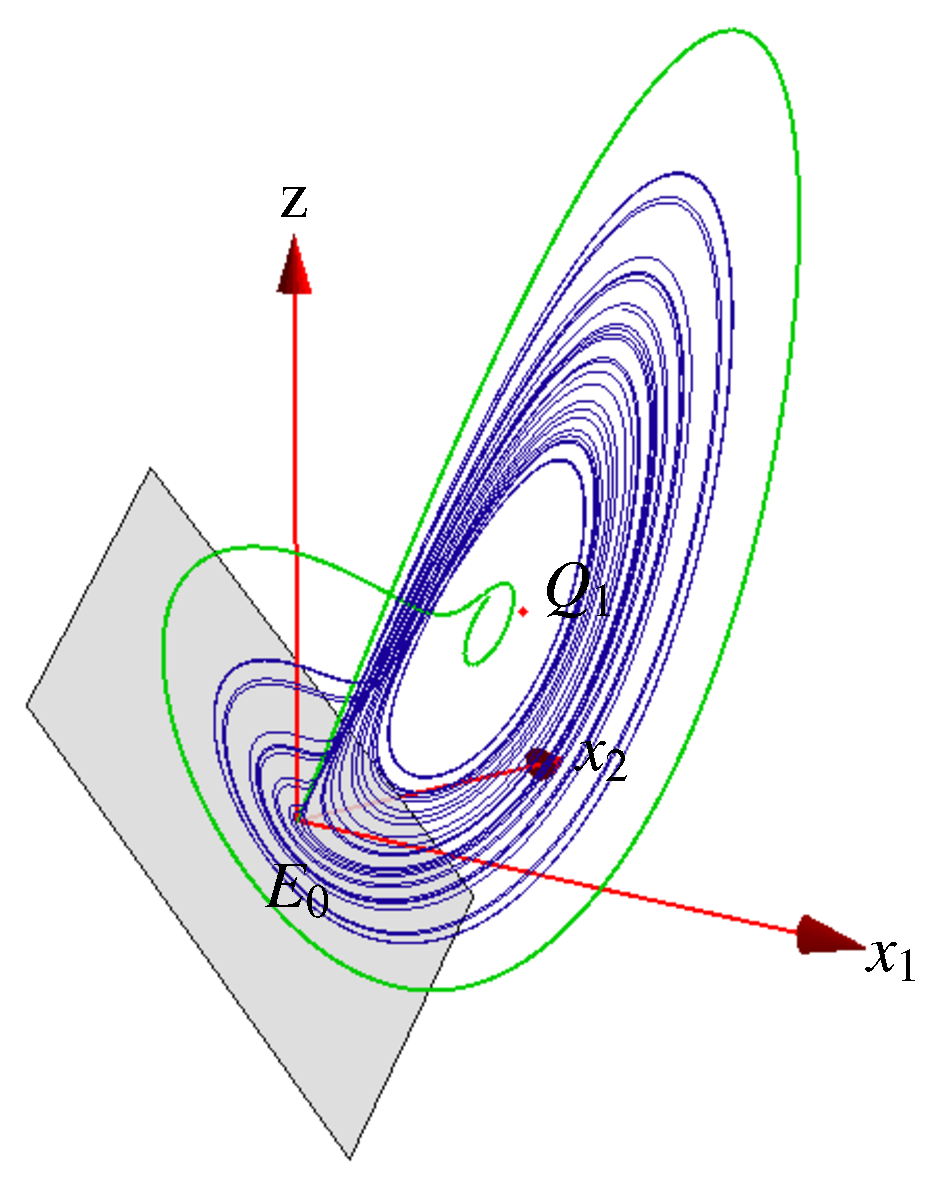
\includegraphics[width=0.35\textwidth,clip=true]{CLEmfAdHoc123}
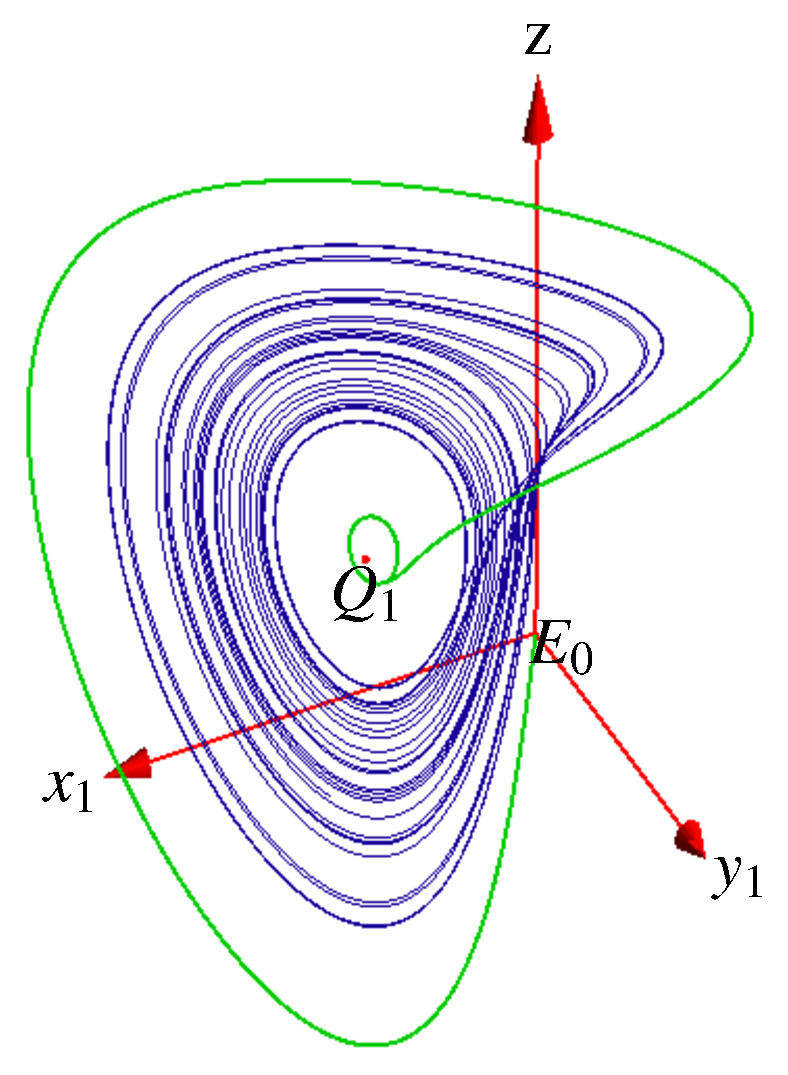
\includegraphics[width=0.35\textwidth,clip=true]{CLEmfAdHoc135}
\end{center}
\caption{
\Statesp\ portraits of \cLf\ in \reducedsp. We use a
moving frame map to a slice orthogonal to the group tangent at
(a) $\slicep  = \ssp_{\REQB{1}}$, with
the gray plane indicating the \sset.
(b) $\slicep  = \ssp_{\REQB{1}}+(0,-5,0,0,0)$,
with the shaded area indicating the \sset.
    }\label{fig:CLEmfsset}
\end{figure}
%%%%%%%%%%%%%%%%%%%%%%%%%%%%%%%%%%%%%%%%%%%%%%%%%%%%%%%%%%%%%%%%
%

\ES{move to discussion:
Rotation of $\ssp$ by angle $\theta$
to the slice defined by \refeq{PCsectQ1} is a linear operation
for any given point and can be applied efficiently
even in a high dimensional space. This is especially true
for truncations of PDEs, when typically the rotation group
representation is a direct sum of irreducible
representations and one is not force to store large matrices.
Of course, the transformation is still non-linear
through the dependence on the angle and equivalent to the
explicit transformations \refeq{eq:invLaser}.
}

\ES{Now mentioned in slice section, merge:
Since rotations commute with time integration, one can take a
different approach: starting with a point on the slice
integrate for small but finite time and then map the
corresponding orbit segment to the section and repeat the
procedure. In this setting it is easier to distinguish
between the two points of intersection of the slice and the
group orbit (for instance we can peek the one with a smaller
clockwise rotation angle into the \slice) but we get no
further practical advantages. Nevertheless, in the limit of
infinitesimal time steps this procedure reveals the
connection of \mframes\ method to its continuous time
counterpart of \refsect{sec:MovFrameODE}.
}
